\section{Materials \& Methods}
\textcolor{red}{\st{The objective of our study was to explore EEG and movement signatures with the potential to detect visual and visuo-tactile conflicts in VR. As such, w}}

\textcolor{n}{The overarching idea of our work is to calibrate a classifier that can be applied online to provide information about the realism underlying the interaction with objects in VR.} \textcolor{n}{To this end,} we designed a study in which participants performed a 3D reach-to-tap task in VR. Our task was inspired by ~\cite{Singh2018-qi}. As a participant reached out to tap an object, they were presented with three sensory feedback modalities (a visual only baseline, visuo-tactile, and visuo-tactile with force-feedback). However, to provoke participants into processing an unrealistic VR interaction, we sometimes provided the feedback prematurely.

% bigger sample
\textcolor{n}{In a previous paper, we reported the results of 10 participants experiencing the force-feedback condition and provided a general description of the PEN in increasing levels of haptic immersion~\cite{Gehrke2019-og}. There, we reported a strength modulation of PEN depending on the haptic channels available for interaction.}

\textcolor{n}{In the current paper, we report data of a significantly larger sample and}\textcolor{red}{\st{In this paper, we}} excluded trials of the visuo-tactile with force-feedback condition. They were only collected for a subset of the participants \textcolor{n}{(10 out of 19)} and were always presented following the counterbalanced conditions of visual only baseline and visuo-tactile. Therefore, the force-feedback condition did not impact the visual only and visuo-tactile contrast. \textcolor{red}{\st{The results including force-feedback are reported in our previous work that provides a description of the PEN in increasing levels of haptic immersion}}~\cite{Gehrke2019-og}. In order to improve \textcolor{red}{\st{state-of-the-art (online)}} \textcolor{n}{real-time} classification using BCI in VR, we leveraged our classification system to localize the network of EEG sources underlying the (linear) separation of unrealistic VR interactions through PEN.

\textcolor{n}{Further, we hypothesized that following the unrealistic situations participants movements are slowed down, indicating a more cautious behavioral approach to the next trial. Therefore, we investigated whether the movement feature `tap time' changed following unrealistic VR interactions.}

\textcolor{red}{\st{In the present work, we leveraged this PEN for classification as well as source localization while also modeling visuo-tactile mismatches using the movement feature `tap time'.}}

\subsection{Apparatus}
The experimental setup, depicted in figure~\ref{setup_and_behavior}a, comprised: (1) a VR headset and a wrist-mounted wearable VIVE tracker, (2) one vibrotactile actuator worn on the fingertip, and (3) a 64-channel EEG system. A medically-compliant EMS device connected via two electrodes was worn on the forearm by a subset of participants, see exclusion statement for this data above.

\textbf{(1) VR and hand tracking.} We used an HTC Vive headset (HTC Corporation, Taoyuan, Taiwan) with the Vive Deluxe Audio Strap and custem EEG cap spacers \footnote{https://grabcad.com/library/adapter-for-vr-eeg-setups-1} to ensure a good fit and less discomfort due to the EEG cap. We used a Vive Tracker, attached to the participant's wrist, to track their right hand. 

\textbf{(2) Vibrotactile feedback.} We used a vibration motor (Model \textit{308-100} from \textit{Precision Microdrives}), which generates 0.8g at 200Hz. This motor measures 8mm in diameter, making it ideal for the fingertip. The vibration feedback was driven at 70mA by a 2N7000 MOSFET, which was connected to an Arduino output pin at 3V.

% \textbf{(3) Force feedback.} We actuated the index finger via electrical muscle stimulation (EMS), which was delivered via two electrodes attached to the participants' \textit{extensor digitorum} muscle. The finger actuation was achieved via a medically-compliant battery powered muscle stimulator (\textit{Rehastim} from \textit{Hasomed}), which provides a maximum of 100mA and is controllable via USB. 

\textbf{(3) EEG Setup.} EEG data was recorded from 64 actively amplified electrodes using BrainAmp DC amplifiers from BrainProducts. Electrodes were placed according to the extended 10\% system ~\cite{Chatrian1985-ys}. After fitting the cap, all electrodes were filled with conductive gel to ensure proper conductivity.

\begin{figure*}[!ht]
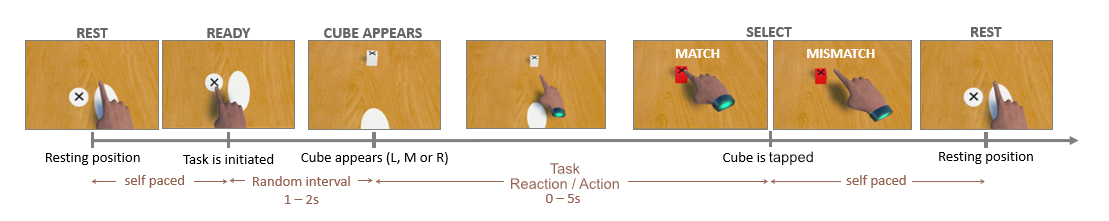
\includegraphics[width=\linewidth]{figures/Task_mismatch.jpg}
\vspace{-15pt}
\caption{Interaction flow depicting one trial in our 3D reach-to-tap task.}
\label{task_flow}
\end{figure*}

\subsection{Task}
Participants performed a 3D reach-to-tap task in VR designed with Unity Software (Unity Technologies, San Francisco, USA). The interaction flow of our task, depicted in Figure~\ref{task_flow}, was as follows: (1) participants moved their hands from the \textit{resting position} to the \textit{ready position}, to indicate they were ready to start the next trial; (2) participants waited for a new target to appear (the time of a new target spawning was randomized between 1-2 s); (3) then, the target (a cube) would appear in one of three possible positions (center, left, right), all equidistant from the participant's \textit{ready position}. \textcolor{n}{A black cross on the top of the cube indicated the location participants were instructed to tap};
(4) then, participants \textcolor{red}{\st{acquired}} \textcolor{n}{completed} the task by moving and tapping the target with their index finger. \textcolor{n}{Tapping success was, at least, indicated by a color change of the cube, see below for a detailed explanation of the feedback conditions.} (5) After a target was \textcolor{red}{\st{acquired}} \textcolor{n}{tapped}, participants moved back to the \textit{resting position}. Here, they could take a break before the next trial.

\textcolor{n}{To maximize EEG data quality, participants were instructed to remain in a calm upright seated position while carrying out the reaching movement. Further, they were instructed to be precise and keep a comfortable pace. However, no feedback was given on the accuracy and speed of their task completion.}

\subsection{Interface conditions}
Participants performed the task in two additive feedback conditions:

(1) \textbf{Visual-only (Visual)}: When participants tapped the cube, it changed its color from white to red (visual feedback.)\\
\indent(2) \textbf{Visual with vibro-tactile (Vibro)}: When participants tapped the cube in the Vibro condition, they received a 100 ms vibro-tactile stimulus with the color change (Visual + vibro-tactile feedback).
% \indent(3) \textbf{visuo-tactile plus force-feedback (EMS)}: in this condition, participants also received a 100 ms of EMS stimulation at the index finger extensor in addition to the visual and vibrotactile feedback (visual + tactile + force feedback)

\textcolor{n}{In this paper, our key focus was the calibration and source localization of a system detecting unrealistic VR interactions such as visual glitches or visuo-haptic synchronization errors. To maximize statistical power for the focus of our investigation we pooled trials from the two interface conditions. In order to build a stimulus-agnostic classification system detecting unrealistic system behavior, we chose to subject the pooled data to the cross-validation-- and localization method.}

\subsection{Introducing Visuo-Haptic Mismatches}
To allow us to compare the event-related EEG and movement signatures in a realistic vs. unrealistic interaction, we presented participants with two different classes of trials: \textbf{match trials (C)} (75\% of the trials) and \textbf{mismatch trials (M)} (25\%). This procedure elicits a prediction mismatch signal in 25\% of the trials similar to previous designs investigating the impact of target probabilities~\cite{Polich2007-cf}.  %on ERP modulations

In the \textbf{matching} trials, the feedback stimuli were presented upon tapping the object, exactly when participants expected them to occur based on the available visual information (finger touching the target in the virtual environment). In contrast, in the \textbf{mismatch} trials, the feedback stimuli were triggered prematurely, which was accomplished by enlarging the invisible radius of tap detection \textcolor{n}{(collision volume around the cube object)} by 350\%. While in the match trials, we used a collision detection volume of the exact size of the VR cube, in the mismatch trials, we used a larger sphere for collision detection. Our enlargement of the collision detecting volume was based on the study design by Singh et al.~\cite{Singh2018-qi}, in which they showed that VR users can detect a visual mismatch at around 200\% of offset from the target. In our pilot tests, we decided to extend the offset to 350\% to make the mismatch more obvious so as to provoke more pronounced prediction errors. 

We used a match-to-mismatch ratio of 75\%-25\% of the total trials by modeling our study after previous studies, which also ensured that participants were faced with a detectable unrealistic behavior of the virtual environment~\cite{Liao2011-po,Wiersema2007-jf,Donchin1988-gq}. For these unrealistic trials to occur, the participants must first be able create a stable model of how the VR world operates, thus the VR world cannot behave at a random 50\%-50\% match-mismatch ratio. 

Finally, these match vs. mismatch trials were presented in five \textcolor{n}{pseudo-}randomly generated sequences. \textcolor{red}{\st{, each with an equal distribution of matches and mismatches.}} \textcolor{n}{Following each mismatch trial, the next trial was always a match trial. To reduce the predictability of when the next mismatch trial would occur, the number of consecutive match trials was pseudo-randomized between 1 and 5.}

\subsection{Experimental design}
The experiment consisted of five phases: (1) a setup phase; (2) a calibration phase; (3) a short training phase; (4) the task itself, in all three possible interface conditions, each followed by a subset of items from the IPQ questionnaire (G1, REAL2, SP4 and INV1)~\cite{Schubert2003-sq} and the NASA-TLX~\cite{Hart1988-iw}. Lastly (5) participants were asked about their experience in the VR and which condition they enjoyed the most.

For training purposes, we asked participants to wear the HTC VIVE VR headset for a maximum of 24 practice trials. Overall, the EEG fitting, calibration, and practice trials took around 30 minutes \textcolor{red}{\st{(with two experimenters)}}. 

Next, we recorded a within-subjects design with 300 trials for each the Visual and Vibro feedback condition. The order of the Visual and Vibro conditions was randomized across participants. \textcolor{n}{We chose to present the two interface conditions in a blocked design. This was done to emphasize the influence of the additional haptic channel while attenuating higher order interactions, such as a prediction error about the upcoming interface condition.}

%%%%% LG writing resources:

% Next, we recorded a within-subjects design with 300 trials for each the Visual and Visuo-Tactile feedback condition, and 100 trials for the EMS condition. The order of the Visual and Visuo-Tactile conditions was randomized across participants with the EMS condition always being the last block. This was done to avoid potential overshadowing of the EMS stimulation (a very strong sensation) on the two other stimulation conditions.

% \subsection{Task and Procedure}
% Using an HTC Vive VR Headset with the Vive Deluxe Audio Strap and a Vive Tracker (HTC Corporation, Taoyuan, Taiwan) attached to the right hand, a 3D object selection task was presented on a virtual table placed on an infinite white plane. The virtual environment was created in the Unity3D engine (Version, company details). White cubes appeared at random either in the center, to the left, or to the right of the participant, equidistant from a starting position (see Figure ??). The time of a new cube spawning was randomized between 1-2 seconds after starting a trial. 

% %no subsections? This so hard to parse, make a task heading or so?
% Participants were tasked to select the cube with their index finger and, upon completion, move their hand back to a resting position indicated on the table. The task was completed in two blocks of 300 trials each, with one block providing visual-only feedback, i.e. the cube changing its color from white to red upon selecting, and one block providing visual-tactile feedback, in which the selection contact was indicated by the color change plus a small vibrotactile pulse. Placed under the index fingertip, a vibration motor (Model \textit{308-100} from \textit{Precision Microdrives}), generating 0.8g at 200Hz and measuring 8mm in diameter was driven at 70mA by a 2N7000 MOSFET connected to an Arduino output pin at 3V. An initial 24 trial training session was followed by the two experimental blocks (balanced across participants), each followed by two questionnaires, NASA-TLX and IPQ. For the main experimental manipulation of asynchrony, 25\% of the trials (totalling 75 asynchronous trials per feedback block of 300 trials) exhibited spatio-temporal asynchrony in line with established oddball paradigms. Object selection was triggered prematurely by bounding a spherical collider to the cube and enlarging it by 350\% in comparison to a collider bounded to the shape of the cube in the synchronous trials. Asynchronous trials were sorted in a pseudo-randomized sequence following synchronous trials, i.e. between one and five synchronous trials preceeded an asynchronous trial. Extended task and apparatus descriptions can be found elsewhere \cite{Gehrke2019}.
% % todo add movie, figure and references